\documentclass[10pt]{amsart} 


\usepackage{amsmath, amssymb, mathrsfs} 

\usepackage[mathscr]{euscript} 
 
\newlength{\mylength}
\setlength{\mylength}{0.25cm}

\usepackage{enumitem}
\setlist{listparindent=\parindent, itemsep=0cm, parsep=\mylength, topsep=0cm}

\usepackage[final]{todonotes}
\usepackage[final]{showkeys} 

\usepackage[breaklinks=true]{hyperref} 
\usepackage{comment} 

\usepackage{graphicx}

\usepackage{url}

\usepackage{tikz-cd}

\usepackage{amsthm}

\makeatletter
\renewenvironment{proof}[1][\proofname]{\par
	\pushQED{\qed}%
	\normalfont \topsep6\p@\@plus6\p@\relax
	\noindent\emph{#1.} 
	\ignorespaces
}{%
\popQED\endtrivlist\@endpefalse
}
\makeatother

\newtheoremstyle{mythm}% name of the style to be used
{\mylength}% measure of space to leave above the theorem. E.g.: 3pt
{0pt}% measure of space to leave below the theorem. E.g.: 3pt
{\itshape}% name of font to use in the body of the theorem
{0pt}% measure of space to indent
{\bfseries}% name of head font
{.\ }% punctuation between head and body
{ }% space after theorem head; " " = normal interword space
{\thmname{#1}\thmnumber{ #2}\thmnote{ (#3)}}

\newtheoremstyle{myrmk}% name of the style to be used
{\mylength}% measure of space to leave above the theorem. E.g.: 3pt
{0pt}% measure of space to leave below the theorem. E.g.: 3pt
{}% name of font to use in the body of the theorem
{0pt}% measure of space to indent
{\itshape}% name of head font
{.\ }% punctuation between head and body
{ }% space after theorem head; " " = normal interword space
{\thmname{#1}\thmnumber{ #2}\thmnote{ (#3)}}

\theoremstyle{mythm} 
%\newtheorem{thm}[subsubsection]{Theorem}
%\newtheorem*{claim}{Claim}
%\newtheorem*{thm}{Theorem} 
\newtheorem{thm}{Theorem}
\newtheorem{lem}[thm]{Lemma} 
\newtheorem{cor}[thm]{Corollary}
\newtheorem{claim}[thm]{Claim}
\newtheorem{prop}[thm]{Proposition}
%\newtheorem*{mthm}{Main Theorem}

%\newtheorem{prop}[subsubsection]{Proposition} 
%\newtheorem*{prop}{Proposition} 
%\newtheorem*{lem}{Lemma}
%\newtheorem*{klem}{Key Lemma}
%\newtheorem*{cor}{Corollary}

\theoremstyle{definition}
%\newtheorem{defn}[subsubsection]{Definition}
\newtheorem*{defn}{Definition} 
\newtheorem{prob}[thm]{Problem}
%\newtheorem{que}[subsubsection]{Question}

\theoremstyle{myrmk} 
%\newtheorem{rmk}[subsubsection]{Remark}
\newtheorem*{rmk}{Remark}
%\newtheorem{note}[subsubsection]{Note} 
\newtheorem*{ex}{Example}

\newcommand{\nc}{\newcommand} 
\nc{\on}{\operatorname}
\nc{\rnc}{\renewcommand} 

\rnc{\setminus}{\smallsetminus} 

\nc{\wt}{\widetilde}
\nc{\wh}{\widehat} 
\nc{\ol}{\overline} 

\nc{\Frob}{\on{Frob}}
\nc{\Gal}{\on{Gal}}

\nc{\BN}{\mathbb{N}}
\nc{\BZ}{\mathbb{Z}}
\nc{\BQ}{\mathbb{Q}}
\nc{\BR}{\mathbb{R}}
\nc{\BC}{\mathbb{C}}

\nc{\id}{\on{id}}
\nc{\Id}{\on{Id}}
\nc{\Tr}{\on{Tr}}

\nc{\la}{\langle}
\nc{\ra}{\rangle} 
\nc{\lV}{\lVert}
\nc{\rV}{\rVert}
\nc{\mb}{\mathbf}
\nc{\mf}{\mathfrak}
%\nc{\cur}{\mathscr}
\nc{\mc}{\mathscr}

\nc{\ira}{\hookrightarrow}
\nc{\hra}{\hookrightarrow}
\nc{\sra}{\twoheadrightarrow} 

\rnc{\Re}{\on{Re}}

\nc{\coker}{\on{coker}}
\nc{\End}{\on{End}}
\rnc{\Im}{\on{Im}}
%\rnc{\Re}{\on{Re}}

\nc{\Hom}{\on{Hom}}

\DeclareMathOperator*{\argmin}{arg\,min}
\DeclareMathOperator*{\argmax}{arg\,max}

\usepackage{marginnote}
\nc{\acts}{\curvearrowright}

\nc{\Mat}{\on{Mat}}

\newenvironment{cd}{\begin{equation*}\begin{tikzcd}}{\end{tikzcd}\end{equation*}\ignorespacesafterend}

\nc{\pfrac}[2]{\frac{\partial #1}{\partial #2}}
\nc{\e}[1]{\begin{align*} #1 \end{align*}}

\usepackage[margin=1in]{geometry}

\makeatletter
\def\blfootnote{\gdef\@thefnmark{}\@footnotetext}
\makeatother

%\renewcommand*{\arraystretch}{1.4}

\setlength{\parskip}{0.25cm}

\definecolor{myblue}{rgb}{0,0.15,0.45}
\newenvironment{myproof}{\color{myblue}\begin{proof}}{\end{proof}} 


\usepackage{bm}

\usepackage{fancyhdr}
\pagestyle{fancy} 
\fancyhead[L]{James Tao}
\fancyhead[C]{18.06 -- Week 11 Recitation}
\fancyhead[R]{Apr.\ 28, 2020}
\fancyfoot[C]{}

\newcounter{part-count}
\setcounter{part-count}{0}

\newenvironment{me}[1]{\begin{enumerate}[#1]\setcounter{enumi}{\value{part-count}}}{\setcounter{part-count}{\value{enumi}}\end{enumerate}}

\nc{\myhead}[1]{\noindent\emph{#1}.}


\begin{document}
	\thispagestyle{fancy}
	
	\color{myblue}
	Sections 6.4 and 6.5 of Strang's book discuss symmetric matrices and their eigenvalues. The book takes an algebraic perspective, giving you various algorithms for computing information about these eigenvalues. In this handout, we explore the geometric aspects of symmetric matrices, starting from the discussion at the end of Section 6.5 (pages 354 and 355) about ellipses, and generalizing to other conic sections and three-dimensional shapes. 
	\color{black}
	
	\section{Quadratic functions in two variables} 
	
	Let's investigate real-valued functions in two variables, of the form
	\[
		f(x, y) = ax^2 + bxy + cy^2. 
	\]
	We could write this as 
	\[
		f(x, y) = \begin{pmatrix}
		x \\ y 
		\end{pmatrix}^\top \underbrace{\begin{pmatrix}
		a & \frac{b}{2} \\ \frac{b}{2} & c
		\end{pmatrix}}_{A}
		\begin{pmatrix}
		x \\ y 
		\end{pmatrix},
	\]
	so every symmetric $2 \times 2$ matrix gives such a function, and vice versa. 
	
	Recall from earlier math classes that $ax^2 + cy^2 = d$ traces out an ellipse or hyperbola depending on the signs of $a, c, d$. The `principal axes' of the conic section are the $x$ and $y$ axis. Considering the more general equation $ax^2 + bxy + cy^2 = d$ (a level set of the function $f(x, y)$ from above) yields `rotated' conic sections, and eigenvectors of $A$ will tell us its principal axes.
	
	\myhead{Example} Consider the symmetric matrix $A = \begin{pmatrix}
	1 & 3 \\ 3 & 1
	\end{pmatrix}$. The function 
	\[
	f(x, y) = \begin{pmatrix}
	x \\ y 
	\end{pmatrix}^\top A \begin{pmatrix}
	x \\ y 
	\end{pmatrix}
	\]
	is then $x^2 + 6xy + y^2$. Contour plot of $f(x, y)$: 
	\begin{center}
		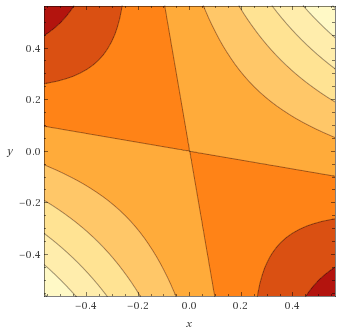
\includegraphics{rec10-pic1} 
	\end{center}
	The function is zero at the origin, positive in the northeast and southwest directions, and negative in the northwest and southeast directions. Its level sets are hyperbolas. 
	
	The eigenvectors of $A$ are $\begin{pmatrix}
	1 \\ 1 
	\end{pmatrix}$ with $\lambda = 4$ and $\begin{pmatrix}
	1 \\ -1
	\end{pmatrix}$ with $\lambda = -2$. Notice that $\begin{pmatrix}
	1 \\ 1 
	\end{pmatrix}$ and $\begin{pmatrix}
	1 \\ -1
	\end{pmatrix}$ are the principal axes of these hyperbolas, and the signs of the eigenvalues tell you whether $f(x, y)$ is \emph{positive} or \emph{negative} in those directions. 
	
	\begin{myproof}
		To prove these geometric statements, let's use the eigenvectors we found to diagonalize $A$. We scale the eigenvectors to be $\begin{pmatrix}
		\frac{1}{\sqrt{2}} \\ \frac{1}{\sqrt{2}}
		\end{pmatrix}$ and $\begin{pmatrix}
		\frac{1}{\sqrt{2}} \\ -\frac{1}{\sqrt{2}} 
		\end{pmatrix}$ so that they are orthonormal. Then the eigenvector matrix 
		\[
			Q = \begin{pmatrix}
			\frac{1}{\sqrt{2}} & \frac{1}{\sqrt{2}} \\ \frac{1}{\sqrt{2}} & - \frac{1}{\sqrt{2}} 
			\end{pmatrix}
		\]
		is orthogonal (and therefore easy to invert). Since the columns of $Q$ are eigenvectors for $A$, we have
		\[
			A = Q \underbrace{\begin{pmatrix}
			4 & 0 \\ 0 & -2
			\end{pmatrix}}_{\Lambda} Q^{\top}
		\]
		where the diagonal matrix contains the eigenvalues $4$ and $-2$. 
		
		Write $\bm{x} = \begin{pmatrix}
		x \\ y
		\end{pmatrix}$ for short. We have 
		\e{
			f(x, y) &= \bm{x}^\top A \bm{X} \\
			&= (Q^\top \bm{x})^\top \Lambda (Q^\top \bm{x}). 
		} 
		So $f(x, y)$ is related to the function 
		\[
			g(x, y) := \bm{x}^\top \Lambda \bm{x}
		\]
		by a coordinate transformation $\bm{x} \mapsto Q^\top \bm{x}$ (which is a rotation around the origin). 
		
		We understand the function $g(x, y)$ because it is just $4x^2 - 2y^2$. Its level sets are hyperbolas, and the principal axes are $\begin{pmatrix}
		1 \\ 0 
		\end{pmatrix}$ and $\begin{pmatrix}
		0 \\ 1
		\end{pmatrix}$, as these point along the $x$ and $y$ axes. Since the $x^2$ coefficient is positive, $g(x, y)$ is positive along $\begin{pmatrix}
			1 \\ 0
		\end{pmatrix}$, and since the $y^2$ coefficient is positive, $g(x, y)$ is negative along $\begin{pmatrix}
		0 \\ 1
		\end{pmatrix}$. 
		
		To transfer these conclusions back to $f(x, y)$, we undo the coordinate transformation by applying $\bm{x} \mapsto Q\bm{x}$. We conclude that the level sets of $f(x, y)$ are also hyperbolas, with principal axes given by $Q \begin{pmatrix}
		1 \\ 0 
		\end{pmatrix}$ and $Q \begin{pmatrix}
		0 \\ 1
		\end{pmatrix}$. These are the columns of $Q$, hence the eigenvectors of $A$. 	
	\end{myproof}
	
	This reasoning works in general. \textbf{The key fact is that any symmetric matrix $A$ has an orthonormal set of eigenvectors with \emph{real} eigenvalues. } Putting these eigenvectors as the columns of an \emph{orthogonal} matrix $Q$, and putting the eigenvalues into a diagonal matrix $\Lambda$, we can thus write 
	\[
		A = Q \Lambda Q^\top. 
	\]
	This allows us to go from a symmetric matrix $A$ to a diagonal matrix $\Lambda$, upon rotating everything by $Q$. 
	
	\myhead{Example}
	Consider the symmetric matrix $A = \begin{pmatrix}
	1 & \frac12 \\
	\frac12 & 1
	\end{pmatrix}$. The function $f(x, y) = \bm{x}^\top A \bm{x}$ is then $x^2 + xy + y^2$. Contour plot of $f(x, y)$: 
	\begin{center}
		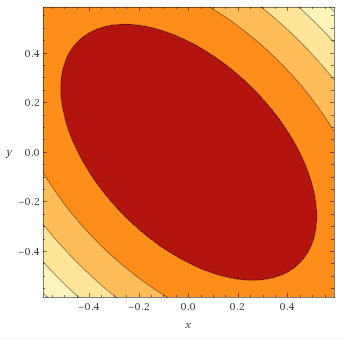
\includegraphics{rec10-pic2}
	\end{center}
	The function is zero at the origin, and positive in all directions.\footnote{Since $f(x, y)$ is `positive in all directions,' we say that $A$ is \emph{positive definite}.} Its level sets are ellipses. 
	
	The eigenvectors of $A$ are $\begin{pmatrix}
	1 \\ 1
	\end{pmatrix}$ with $\lambda = \frac32$ and $\begin{pmatrix}
	1 \\ -1
	\end{pmatrix}$ with $\lambda = \frac12$. The eigenvectors give the principal axes of the ellipses, and the signs of the eigenvalues tell you that $f(x, y)$ is positive in both of those directions. 
	
	\myhead{Example}
	Consider the symmetric matrix $A = \begin{pmatrix}
	1 & 1 \\
	1 & 1
	\end{pmatrix}$. The function $f(x, y) = \bm{x}^\top A \bm{x}$ is then $x^2 + 2xy + y^2 = (x+y)^2$. Contour plot of $f(x, y)$: 
	\begin{center}
		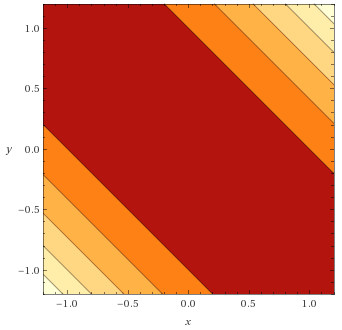
\includegraphics{rec10-pic3}
	\end{center}
	The function is zero at the origin, constant along the northwest/southeast directions, and positive along the northeast/southwest directions. 
	
	The eigenvectors of $A$ are $\begin{pmatrix}
	1 \\ 1
	\end{pmatrix}$ with $\lambda = 2$ and $\begin{pmatrix}
	1 \\ -1
	\end{pmatrix}$ with $\lambda = 0$. The $\lambda = 2$ eigenvalue tells you that the function is positive in the direction of the first eigenvector, while the $\lambda = 0$ eigenvalue tells you that the function is zero in the direction of the second eigenvector. Since $f(x, y)$ is always nonnegative (but can be zero away from the origin), we say that $A$ is \emph{positive semidefinite}. 
	
	\section{Quadratic functions in three variables} 
	
	\myhead{Problem}
	Consider the symmetric matrix $A = \begin{pmatrix}
	1 & \frac12 & 0 \\
	\frac12 & 1 & 0 \\
	0 & 0 & 2
	\end{pmatrix}$. It defines the function 
	\e{
		f(x, y, z) &= \bm{x}^\top A \bm{x} \\
		&= x^2 + y^2 + 2z^2 + xy. 
	} 
	The equation $f(x, y, z) = 1$ specifies the following ellipsoid: 
	\begin{center}
		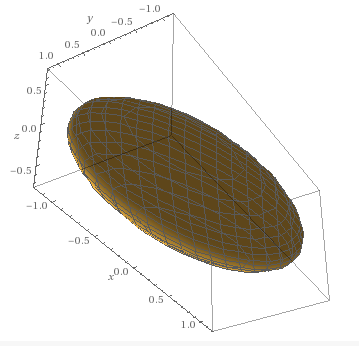
\includegraphics{rec10-pic4}
	\end{center}
	Draw (on this picture) the three principal axes of the ellipsoid, which are the eigenvectors of $A$. Which eigenvector of $A$ has the largest eigenvalue, and which one has the smallest? How would you write down a matrix $Q$ which would `un-rotate' this ellipsoid? 
	
	\myhead{Problem}
	Consider the symmetric matrix $A = \begin{pmatrix}
	1 & \frac12 & 0 \\
	\frac12 & 1 & 2 \\
	0 & 2 & 2
	\end{pmatrix}$. It defines the function 
	\e{
		f(x, y, z) &= \bm{x}^\top A \bm{x} \\
		&= x^2 + y^2 + 2z^2 + xy + 4yz. 
	} 
	The equation $f(x, y, z) = 1$ specifies the following one-sheeted hyperboloid: 
	\begin{center}
		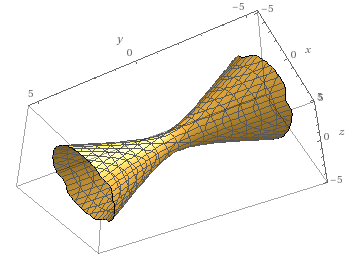
\includegraphics{rec10-pic5}
	\end{center}
	Draw (on this picture) the three principal axes of the hyperboloid, which are the eigenvectors of $A$. How many positive (resp.\ negative) eigenvalues does $A$ have? Which eigenvectors have positive eigenvalues? In what region of space is $f(x, y, z)$ positive (resp.\ negative)? 
	
	It may be helpful to refer to this plot of the equation $f(x, y, z) = 0$: 
	
	\begin{center}
		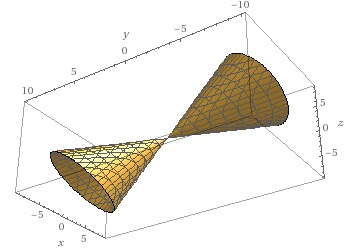
\includegraphics{rec10-pic8}
	\end{center}
	
	\myhead{Problem}
	Consider the symmetric matrix $A = \begin{pmatrix}
	-1 & \frac12 & 0 \\
	\frac12 & -1 & 2 \\
	0 & 2 & -2
	\end{pmatrix}$. It defines the function 
	\e{
		f(x, y, z) &= \bm{x}^\top A \bm{x} \\
		&= -x^2 - y^2 - 2z^2 + xy + 4yz. 
	} 
	The equation $f(x, y, z) = 1$ specifies the following two-sheeted hyperboloid: 
	\begin{center}
		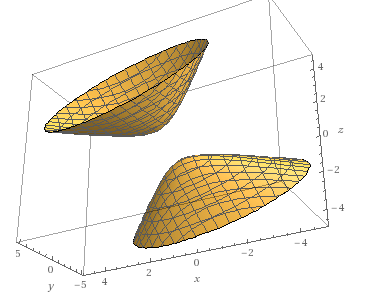
\includegraphics{rec10-pic6}
	\end{center}
	Draw (on this picture) the three principal axes of the hyperboloid, which are the eigenvectors of $A$. How many positive (resp.\ negative) eigenvalues does $A$ have? Which eigenvectors have positive eigenvalues? 
	
	\myhead{Problem}
	Consider the symmetric matrix $A = \begin{pmatrix}
	1 & -\frac12 & 0 \\
	-\frac12 & 1 & -2 \\
	0 & -2 & \frac{16}{3}
	\end{pmatrix}$. It defines the function 
	\e{
		f(x, y, z) &= \bm{x}^\top A \bm{x} \\
		&= x^2 + y^2 + \frac{16}{3} \, z^2 - xy - 4yz. 
	} 
	The equation $f(x, y, z) = 1$ specifies the following (elliptic) cylinder: 
	\begin{center}
		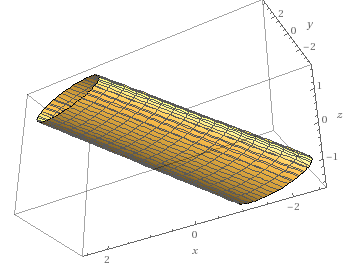
\includegraphics{rec10-pic7}
	\end{center}
	Draw (on this picture) the three principal axes of the cylinder, which are the eigenvectors of $A$. What are the signs of the eigenvalues of $A$? What is the determinant of $A$? Is $A$ positive semidefinite or positive semidefinite? 
	
	\myhead{Problem} 
	For each function considered in the previous problems, determine the points $\bm{x}$ on the unit sphere (centered at the origin) which maximize $f(\bm{x})$. Suppose one travels from the origin in a randomly chosen direction---how would you figure out if the function is more likely to increase or decrease? 
	
	Questions of this sort are useful in optimization. 
	
	
	
	
	
	
		
	
	
	
	
	
	
	
	
\end{document} 